\section{System of particles}
Consider $n$ particles of masses $ m_i $, positions $ \bfr_i(t) $ and momentum $ \bfp_i(t) = m_i \dot{\bfr}_i $. Newton's 2nd law applies to the $i$th particle individually: 
\[
    m_i \ddot{\bfr}_i = \dot{\bfp}_i = \bfF_i,
\]
where $\bfF_i$ is total force applied to the $i$th particle. Distinguish between external and internal forces: 
\[
    \bfF_i = \bfF_i^{\text{ext}}+\sum_{j\neq i}\bfF_{ij},
\]
where $\bfF_{ij}$ is the force applied to the $ i $th particle by the $j$th particle and $ \bfF_i^{\text{ext}} $ is the external force exerted to the $i$th particle.

By Newton's 3rd law, $ \bfF_{ij}=-\bfF_{ji} $, which can be checked in gravity.

\subsection{Centre of mass}
Consider $n$ particles with total mass $ M=\sum_{i=1}^{n}m_i $. The \textbf{centre of mass} is located at 
\[
    \bfR = \frac{1}{M} \sum_{i=1}^{n} m_i \mathbf{r}_i.
\]
Consider the total linear momentum: 
\[
    \bfP = \sum_{i=1}^{n} m_i \dot{\bfr}_i = \sum_{i=1}^{n} \bfp_i = M \dot{\bfR},
\]
i.e. total linear momentum is equivalent to that of a point mass $M$ located at $\bfR$. Then 
\[
    \dot{\bfP} = M \ddot{\bfR} = \sum_{i=1}^{n}\dot{\bfp}_i = \sum_{i=1}^{n} \bfF_i^{\text{ext}}+\sum_{i=1}^{n}\sum_{j\neq i}\bfF_{ij}\footnote{By considering parwise sums, $\sum_{i=1}^{n}\sum_{j\neq i}\bfF_{ij}=\mathbf{0}$.} =\bfF^{\text{ext}} .
\]
i.e. centre of mass moves as if it is the position of a mass $M$ under the influence of a force $ \bfF^{\text{ext}} $, extending Newton's 2nd law to a system of particles. If $ \bfF^{\text{ext}}=\mathbf{0} $ then $ \dot{\bfP}=\mathbf{0} $ and thus total momentum is conserved. There will be a ``centre of mass'' frame with origin at $ \bfR $, which is inertial. In this frame $ \dot{\bfR}=\mathbf{0} $, e.g. take $ \bfR=\mathbf{0} $.

\subsection{Motion relative to centre of mass}
Let $ \bfr_i = \bfR+\bfs_i $, where $\bfs_i$ are position vectors relative to centre of mass. Note that 
\[
    \sum_{i=1}^{n}m_i\bfs_i = \sum_{i=1}^{n}m_i(\bfr_i-\bfR) = \sum_{i=1}^{n}m_i\bfr_i-\bfR \sum_{i=1}^{n}m_i = \mathbf{0},
\]
so 
\[
    \frac{\mathrm{d}}{\mathrm{d}t} \sum_{i=1}^{n} m_i \bfs_i = \mathbf{0}. 
\]
The total linear momentum is 
\[
    \bfP = \sum_{i=1}^{n}m_i (\dot{\bfR}+\dot{\bfs}_i) = \sum_{i=1}^{n}m_i \dot{\bfR} = M \dot{\bfR},
\]
which is indeed consistent.

\subsection{Angular momentum}
Total angular momentum about origin is 
\[
    \bfL = \sum_{i=1}^{n} \bfr_i \times \bfp_i,
\]
so
\begin{align*}
    \dot{\bfL} &= \sum_{i=1}^{n}\dot{\bfr}_i \times \bfp_i + \sum_{i=1}^{n} \bfr_i \times \dot{\bfp}_i = \sum_{i=1}^{n} \bfr_i \times \dot{\bfp}_i\\ 
    &= \sum_{i=1}^{n}\mathbf{r}_i \times \bfF_i^{\text{ext}}+\sum_{i=1}^{n}\mathbf{r}_i \times \sum_{j=1}^{n}\bfF_{ij}\\ 
    &= \sum_{i=1}^{n}\mathbf{r}_i \times \bfF_i^{\text{ext}}+\frac{1}{2}\sum_{i,j=1}^{n} (\bfr_i-\bfr_j)\times \bfF_{ij}.
\end{align*}
The latter is $\mathbf{0}$ if, e.g. $ \bfF_{ij}\parallel \bfr_i-\bfr_j $. In this case 
\[
    \dot{\bfL} = \sum_{i=1}^{n}\mathbf{r}_i \times \bfF_i^{\text{ext}} = \bfG^{\text{ext}},
\]
the total external torque acting on the system.

Relative to the centre of mass, total angular momentum is given by 
\begin{align*}
    \bfL &= \sum_{i=1}^{n} m_i(\bfR+\bfs_i) \times (\dot{\bfR}+\dot{\bfs}_i)\\ 
    &= \sum_{i=1}^{n}m_i (\bfR \times \dot{\bfR})+\sum_{i=1}^{n}m_i \bfs_i \times \dot{\bfs}_i.
\end{align*}
This is the angular momentum of a particle of mass $M$ at $ \bfR $ moving with velocity $ \dot{\bfR} $ and angular momentum associsated with motion of particles relative to the centre of mass.

\subsection{Energy}
Total kinetic energy $T$ is 
\begin{align*}
    T &= \sum_{i=1}^{n}\frac{1}{2}m_i \dot{\bfr}_i^2 = \sum_{i=1}^{n} \frac{1}{2}m_i (\dot{\bfR}+\dot{\bfs}_i)^2\\ 
    &= \frac{1}{2} \dot{\bfR}^2 \sum_{i=1}^{n}m_i+\frac{1}{2}\sum_{i=1}^{n}m_i \dot{\bfs}_i^2,
\end{align*}
which is the KE of a particle of mass $M$ with velocity $ \dot{\bfR} $. KE is associsated with particle motions relative to the centre of mass.

Is energy conserved? Consider 
\begin{align*}
    \frac{\mathrm{d}T}{\mathrm{d}t} &= \frac{\mathrm{d}}{\mathrm{d}t}\sum_{i=1}^{n}\frac{1}{2}m_i \dot{\bfr}_i^2 = \sum_{i=1}^{n}m_i \dot{\bfr}_i \cdot \ddot{\bfr}_i\\
    &= \sum_{i=1}^{n} \dot{\bfr}_i \cdot \bfF_i^{\text{ext}}+\sum_{i=1}^{n}\dot{\bfr}_i \cdot \sum_{j=1}^{n}\bfF_{ij}\\ 
    &= \sum_{i=1}^{n} \dot{\bfr}_i \cdot \bfF_i^{\text{ext}}+ \sum_{j>i} (\dot{\bfr}_i-\dot{\bfr}_j)\cdot \bfF_{ij}.
\end{align*}
If external forces are defined by a potential 
\[
    \bfF_{i}^{\text{ext}} = - \nabla_{\bfr_i} V_i^{\text{ext}},
\]
and internal forces are defined by a potential 
\[
    \bfF_{ij} = -\nabla _{\bfr_i} V(\bfr_i-\bfr_j),
\]
we get 
\[
    \frac{\mathrm{d}T}{\mathrm{d}t} = - \frac{\mathrm{d}}{\mathrm{d}t}\sum_{i=1}^{n}V^{\text{ext}}(\bfr_i) - \frac{\mathrm{d}}{\mathrm{d}t}\sum_{i=1}^{n}\sum_{j>i} V(\bfr_i-\bfr_j).
\]
i.e. we have conservation of energy if the above conditions hold.

\subsection{Two body problem}
Consider two particles with no external force acting. The centre of mass is at 
\[
    \bfR = \frac{1}{M}(m_1\bfr_1+m_2\bfr_2).
\]
\begin{center}
    \begin{tikzpicture}[rotate=30]
      \node [dot] {};
      \node [anchor = south east] {$\mathbf{r}_2$};
  
      \node at (3, 0) [dot, minimum size = 4] {};
      \node at (3, 0) [anchor = south east] {$\mathbf{r}_1$};
  
      \node at (2, 0) [dot, minimum size = 3] {};
      \node at (2, 0) [anchor = south east] {$\mathbf{R}$};
      \draw [->-=0.5] (0, 0) -- (3, 0) node [pos =0.5, anchor = south east] {$\mathbf{r}$};
    \end{tikzpicture}
\end{center}
The separation vector between these 2 particles is $ \bfr=\bfr_1-\bfr_2. $ Since $ \bfF^{\text{ext}}=0, \ddot{\bfR}=\mathbf{0} $. Hence CoM moves with constant velocity. Note that 
\[
    \ddot{\bfr} = \ddot{\bfr}_1-\ddot{\bfr}_2 = \frac{\bfF_{12}}{m_1}-\frac{\bfF_{21}}{m_2} = \left( \frac{1}{m_1}+\frac{1}{m_2} \right)\bfF_{12} ,
\]
equivalently 
\[
    \mu \ddot{\bfr} = \bfF_{12},\quad \mu = \frac{m_1m_2}{m_1+m_2}.
\]
$ \mu $ is called the ``reduced mass'' (note that $ \mu<m_1,\mu<m_2 $). This is the standard Newton's 2nd law to a particle of mass $ \mu $.

Now consider gravitational force: 
\[
    \mu \ddot{\bfr} = -\frac{Gm_1m_2}{|\bfr|^3}\bfr \Longrightarrow \ddot{\bfr} = -G(m_1+m_2)\frac{\bfr}{|\bfr|^3}.
\]
This is the motion of a particle under effect of gravitational force due to mass $ M=m_1+m_2 $ fixed at the \textit{origin}.

Consider Earth-Sun orbit: both move about the centre of mass, both orbits have the same shape, but the sizes of orbits are different. Ratio of masses Earth/Sun is $ 3\times 10^{-4} $, Earth-Sun orbit is about $ 1.5\times 10^7 \mathrm{km} $, hence Sun's displacement is about $ 450\mathrm{km} $.

It can be shown that
\begin{align*}
  \mathbf{L} &= M\mathbf{R} \times \dot{\mathbf{R}} + \mu \mathbf{r}\times \dot{\mathbf{r}}\\
  T &= \frac{1}{2} M|\dot{\mathbf{R}}|^2 + \frac{1}{2}\mu |\dot{\mathbf{r}}|^2
\end{align*}
by expressing $\mathbf{r}_1$ and $\mathbf{r}_2$ in terms of $\mathbf{r}$ and $\mathbf{R}$.

\subsection{Variable-mass problem}
All systems we've studied so far have fixed mass. However, in real life, many objects have changing mass, such as rockets, fireworks, falling raindrops and rolling snowballs.

Again, we will use Newton's second law, which states that
\[
  \frac{\rmd \mathbf{p}}{\rmd t} = \mathbf{F},\quad\text{with }\mathbf{p} = m\dot{\mathbf{r}}.
\]
We will consider a rocket moving in one dimension with mass $m(t)$ and velocity $v(t)$. The rocket propels itself forwards by burning fuel and ejecting the exhaust at velocity $-u$ relative to the rocket.

At time $t$, the rocket looks like this:
\begin{center}
  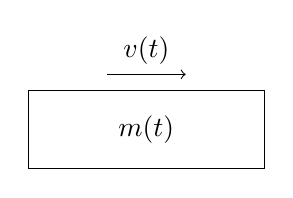
\begin{tikzpicture}
    \draw (0, 0.5) rectangle (3, -0.5);
    \node at (1.5, 0) {$m(t)$};
    \draw [->] (1, 0.7) -- (2, 0.7) node [pos = 0.5, above] {$v(t)$};
  \end{tikzpicture}
\end{center}
At time $t + \delta t$, it ejects exhaust of mass $m(t) - m(t + \delta t)$ with velocity $v(t) - u + O(\delta t)$.
\begin{center}
  \begin{tikzpicture}
    \draw (0, 0.5) rectangle (3, -0.5);
    \node at (1.5, 0) {$m(t)$};
    \draw [->] (1, 0.7) -- (2, 0.7) node [pos = 0.5, above] {$v(t)$};
    \node at (-1, 0) [dot] {$m$};
    \draw [->] (-1.33, 0) -- (-2, 0) node [left] {$v(t) - u$};
  \end{tikzpicture}
\end{center}
The change in total momentum of the system (rocket + exhaust) is
\begin{align*}
  \delta p &= m(t + \delta t)v(t + \delta t) + [m(t) - m(t + \delta t)][v(t) - u(t) + O(\delta t)] - m(t)v(t)\\
  &= (m + \dot{m}\delta t + O(\delta t^2))(v + \dot{v} \delta t + O(\delta t^2)) - \dot{m}\delta t(v - u) + O(\delta t^2) - mv\\
  &= (\dot{m}v + m\dot{v} - \dot{m}v + \dot{m}u)\delta t + O(\delta t^2)\\
  &= (m\dot{v} + \dot{m}u)\delta t + O(\delta t^2).
\end{align*}
Newton's second law gives
\[
  \lim_{\delta \to 0} \frac{\delta p}{\delta t} = F
\]
where $F$ is the external force on the rocket. So we obtain
\begin{proposition}[Rocket equation]
  \[
    m\frac{\rmd v}{\rmd t} + u\frac{\rmd m}{\rmd t} = F.
  \]
\end{proposition}
\begin{example}
  Suppose that we travel in space with $F = 0$. Assume also that $u$ is constant. Then we have
  \[
    m\frac{\rmd v}{\rmd t} = -u\frac{\rmd m}{d t}.
  \]
  So
  \[
    v = v_0 + u \log \left(\frac{m_0}{m(t)}\right),
  \]
  Note that we are expressing things in terms of the mass remaining $m$, not time $t$.

  Note also that the velocity does not depend on the rate at which mass is ejected, only the velocity at which it is ejected. Of course, if we expressed $v$ as a function of time, then the velocity at a specific time \emph{does} depend on the rate at which mass is ejected.
\end{example}

\begin{example}
  Consider a falling raindrop of mass $m(t)$, gathering mass from a stationary cloud. In this case, $u = v$. So
  \[
    m\frac{\rmd v}{\rmd t} + v\frac{\rmd m}{\rmd t} = \frac{\rmd }{\rmd t}(mv) = mg,
  \]
  with $v$ measured downwards. To obtain a solution of this, we will need a model to determine the rate at which the raindrop gathers mass.
\end{example}